\documentclass[a4paper,12pt]{article}
\usepackage[margin=18mm]{geometry}
\usepackage{tikz}
\usepackage{amsmath}
\usepackage{xcolor}
\newcommand{\pFourCell}[2]{\makebox[#1em][c]{\ensuremath{#2}}}
\newcommand{\pFourCenterBox}[1]{\begingroup\setbox0=\hbox{$\displaystyle #1$}\dimen0=\ht0\advance\dimen0 by -\dp0\divide\dimen0 by 2\lower\dimen0\box0\endgroup}
\newdimen\pFourFractionRuleThickness
\pFourFractionRuleThickness=0.4pt
\newcommand{\pFourTopAlign}[3]{\raisebox{-#1}[0pt][\dimexpr #1 + #2\relax]{\ensuremath{\displaystyle #3}}}
\newcommand{\pFourBottomAlign}[3]{\raisebox{#2}[\dimexpr #1 + #2\relax][0pt]{\ensuremath{\displaystyle #3}}}
\newcommand{\pFourFractionInner}[2]{\hbox to #1{\hss$\displaystyle #2$\hss}}
\newcommand{\pFourFractionC}[4]{\begingroup\color{#1}\genfrac{}{}{\pFourFractionRuleThickness}{0}{\raisebox{0.14em}{\pFourFractionInner{#2}{{\color{black}#3}}}}{\raisebox{-0.18em}{\pFourFractionInner{#2}{{\color{black}#4}}}}\endgroup}
\newcommand{\pFourFraction}[3]{\genfrac{}{}{\pFourFractionRuleThickness}{0}{\raisebox{0.14em}{\pFourFractionInner{#1}{#2}}}{\raisebox{-0.18em}{\pFourFractionInner{#1}{#3}}}}
\newcommand{\pFourRootC}[2]{\begingroup\setbox0=\hbox{$\displaystyle #2$}\setbox2=\hbox{$\displaystyle \sqrt{\phantom{\copy0}}$}\dimen0=\wd2\advance\dimen0 by -\wd0\hbox{\rlap{\textcolor{#1}{\copy2}}\kern\dimen0\box0}\endgroup}
\newcommand{\pFourRoot}[1]{\pFourRootC{black}{#1}}
\newcommand{\pFourRootDegreeC}[3]{\begingroup\setbox0=\hbox{$\displaystyle #3$}\setbox2=\hbox{$\displaystyle \sqrt[#2]{\phantom{\copy0}}$}\dimen0=\wd2\advance\dimen0 by -\wd0\hbox{\rlap{\textcolor{#1}{\copy2}}\kern\dimen0\box0}\endgroup}
\newcommand{\pFourRootDegree}[2]{\pFourRootDegreeC{black}{#1}{#2}}
\pagestyle{empty}
\begin{document}

\section*{Spaltentreue LaTeX-Ausgabe}
\noindent Gleichung: \texttt{B}\texttt{\textasciicircum{}(2*}\texttt{x}\texttt{-1)=}\texttt{y}\texttt{/}\texttt{a}\texttt{  ->  2*}\texttt{x}\texttt{-1=}\texttt{log}\texttt{\_}\texttt{B}\texttt{(}\texttt{y}\texttt{/}\texttt{a}\texttt{)} \hfill Zielvariable: \texttt{x} \hfill Profil: \texttt{standard}

\vspace{8mm}
\begin{center}
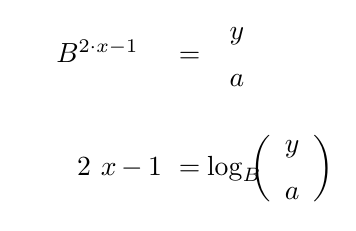
\begin{tikzpicture}[x=1em,y=-1em]
\node[anchor=base, inner sep=0pt] at (2.52,2.7) {$\pFourCell{5.04}{B^{{\scriptstyle 2\cdot{}x-1}}}$};
\node[anchor=base, inner sep=0pt] at (7.56,2.7) {$\pFourFraction{1.8em}{\makebox[1.8em][c]{\ensuremath{\pFourCell{0.9}{y}}}}{\makebox[1.8em][c]{\ensuremath{\pFourCell{0.9}{a}}}}$};
\node[anchor=base, inner sep=0pt] at (5.85,2.7) {$\pFourCell{1.62}{=}$};
\node[anchor=base, inner sep=0pt] at (9.56,6.78) {$\pFourFraction{1.8em}{\makebox[1.8em][c]{\ensuremath{\pFourCell{0.9}{y}}}}{\makebox[1.8em][c]{\ensuremath{\pFourCell{0.9}{a}}}}$};
\node[anchor=base, inner sep=0pt] at (2.04,6.78) {$\pFourCell{0.88}{2}$};
\node[anchor=base, inner sep=0pt] at (2.93,6.78) {$\pFourCell{0.9}{x}$};
\node[anchor=base, inner sep=0pt] at (3.77,6.78) {$\pFourCell{0.78}{-}$};
\node[anchor=base, inner sep=0pt] at (4.6,6.78) {$\pFourCell{0.88}{1}$};
\node[anchor=base, inner sep=0pt] at (5.85,6.78) {$\pFourCell{1.62}{=}$};
\node[anchor=base, inner sep=0pt] at (7.47,6.78) {$\pFourCell{1.62}{\pFourCell{1.62}{\log_{B}}}$};
\node[anchor=base, inner sep=0pt] at (8.47,6.78) {$\pFourCell{0.38}{\left(\rule[-1em]{0pt}{1.96em}\right.}$};
\node[anchor=base, inner sep=0pt] at (10.65,6.78) {$\pFourCell{0.38}{\left.\rule[-1em]{0pt}{1.96em}\right)}$};
\end{tikzpicture}
\end{center}

\end{document}
